\chapter{项目展示}

\section{教程版块}

用户可以查看公开的以及分享给自己的教程,教程的可读权限和可写权限是在创建教程时给定的。教程支持Markdown和Latex渲染,用户可以方便地插入标题、代码块等基本元素。PhoeniX支持在教程中嵌入程序的可执行环境,用户无需打开IDE即可运行程序。教程详情页面如下:

\begin{figure}[H]
    \centering
    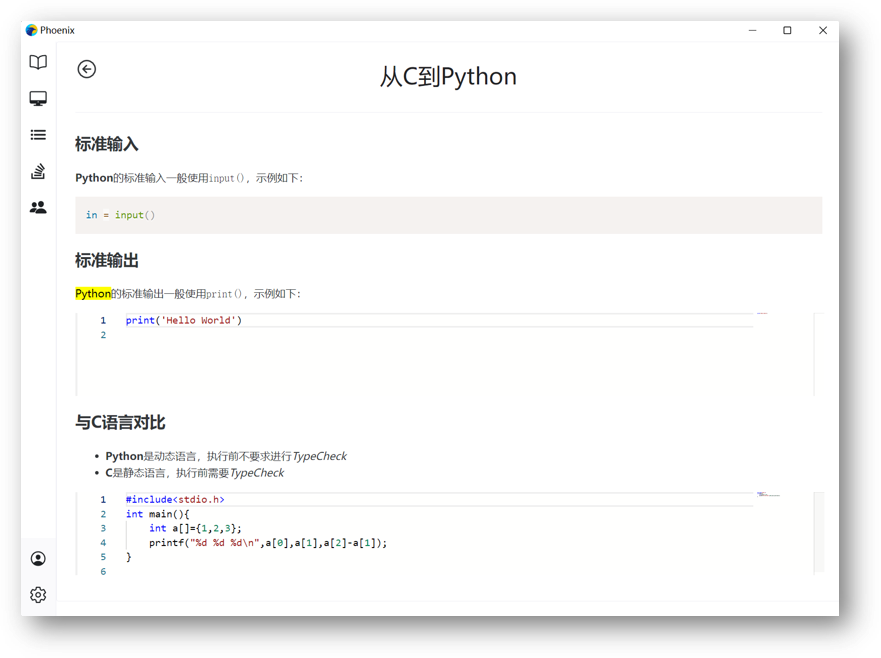
\includegraphics[width=0.7\textwidth]{figure/tutorial1.png}
    \caption{\textbf{教程详情页面}}
    \label{fig:tutorial1}
\end{figure}

\section{评测版块}

用户可以设计并上传自己的题目,并查看具有可读权限的所有题目。用户的题目列表中会标明题目的难度、名称、通过情况等信息,方便用户进行筛选,题目列表页面如下:

\begin{figure}[H]
    \centering
    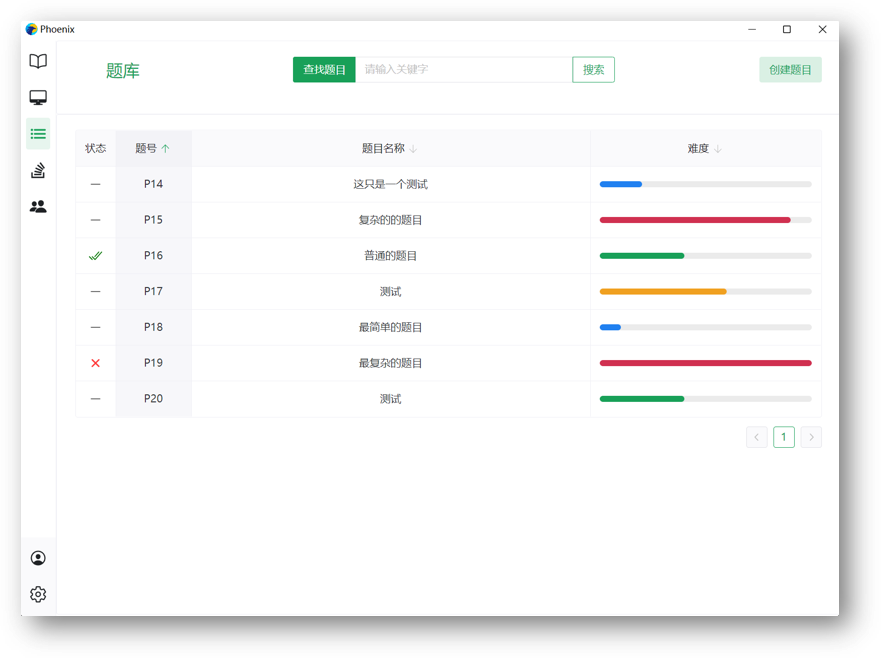
\includegraphics[width=0.7\textwidth]{figure/problem1.png}
    \caption{\textbf{题目列表页面}}
    \label{fig:problem1}
\end{figure}

对于每一个题目,用户都可以查看自己的历史评测记录。在历史评测记录中会显示用户所用的编程语言、评测结果、评测时间等信息。用户可以下载自己的历史评测文件,评测记录页面如下:

\begin{figure}[H]
    \centering
    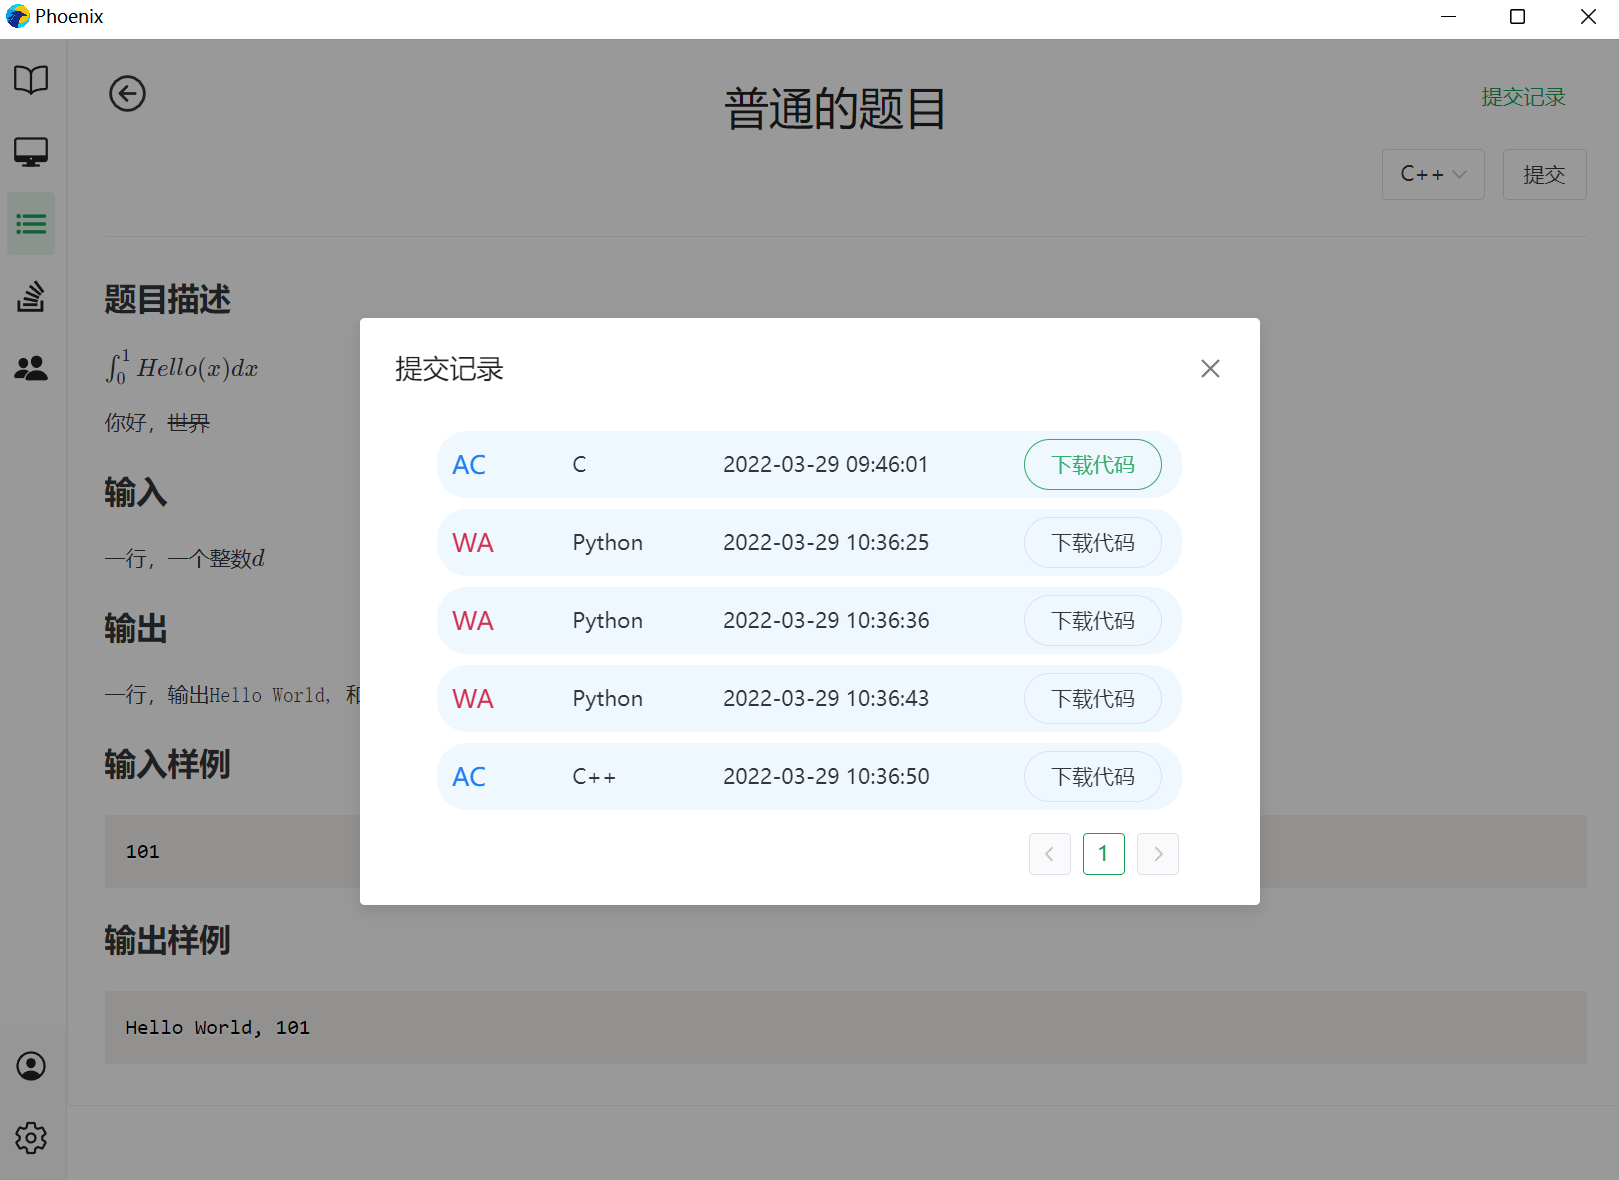
\includegraphics[width=0.7\textwidth]{figure/problem2.png}
    \caption{\textbf{评测记录页面}}
    \label{fig:problem2}
\end{figure}

\section{组织管理版块}

用户可以自发地创建组织并邀请其他用户加入,实时查看自己收到的组织邀请,并方便地查看自己所属的所有组织,组织列表页面如下:

\begin{figure}[H]
    \centering
    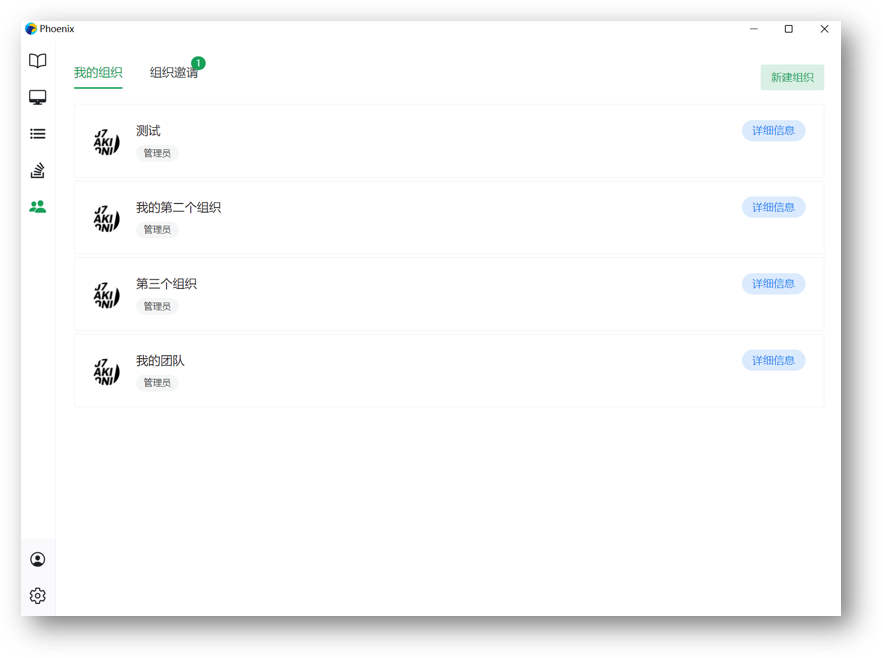
\includegraphics[width=0.7\textwidth]{figure/team1.png}
    \caption{\textbf{组织列表页面}}
    \label{fig:team1}
\end{figure}

组织创建者可以将一些组织成员设置为组织管理员。组织管理员可以设置组织的相关信息(例如组织简介等),在组织内共享题目和教程,创建组织范围内的比赛等。组织管理页面如下:

\begin{figure}[H]
    \centering
    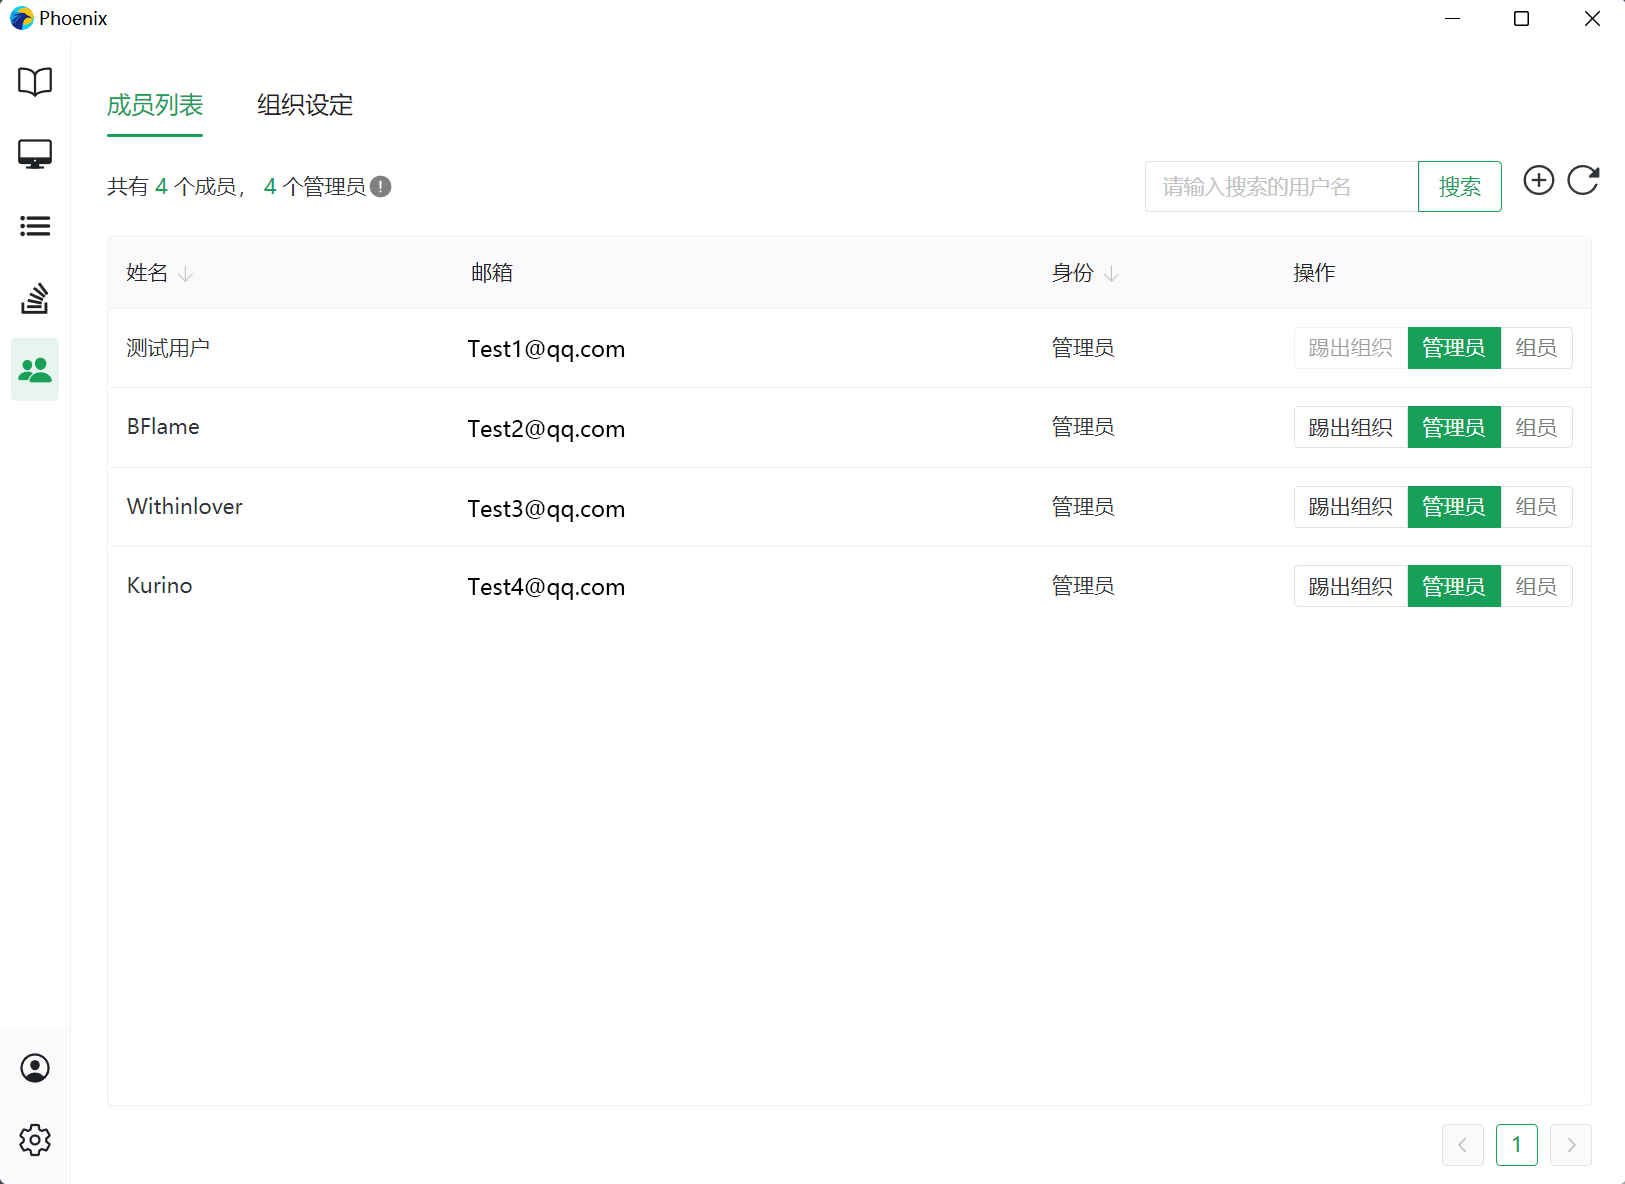
\includegraphics[width=0.7\textwidth]{figure/team2.png}
    \caption{\textbf{组织管理页面}}
    \label{fig:team2}
\end{figure}

\section{比赛版块}

组织管理员可以通过选择题目创建比赛,比赛可以指定允许参加比赛的用户范围、比赛开启的时间等内容,创建比赛页面如下:

\begin{figure}[H]
    \centering
    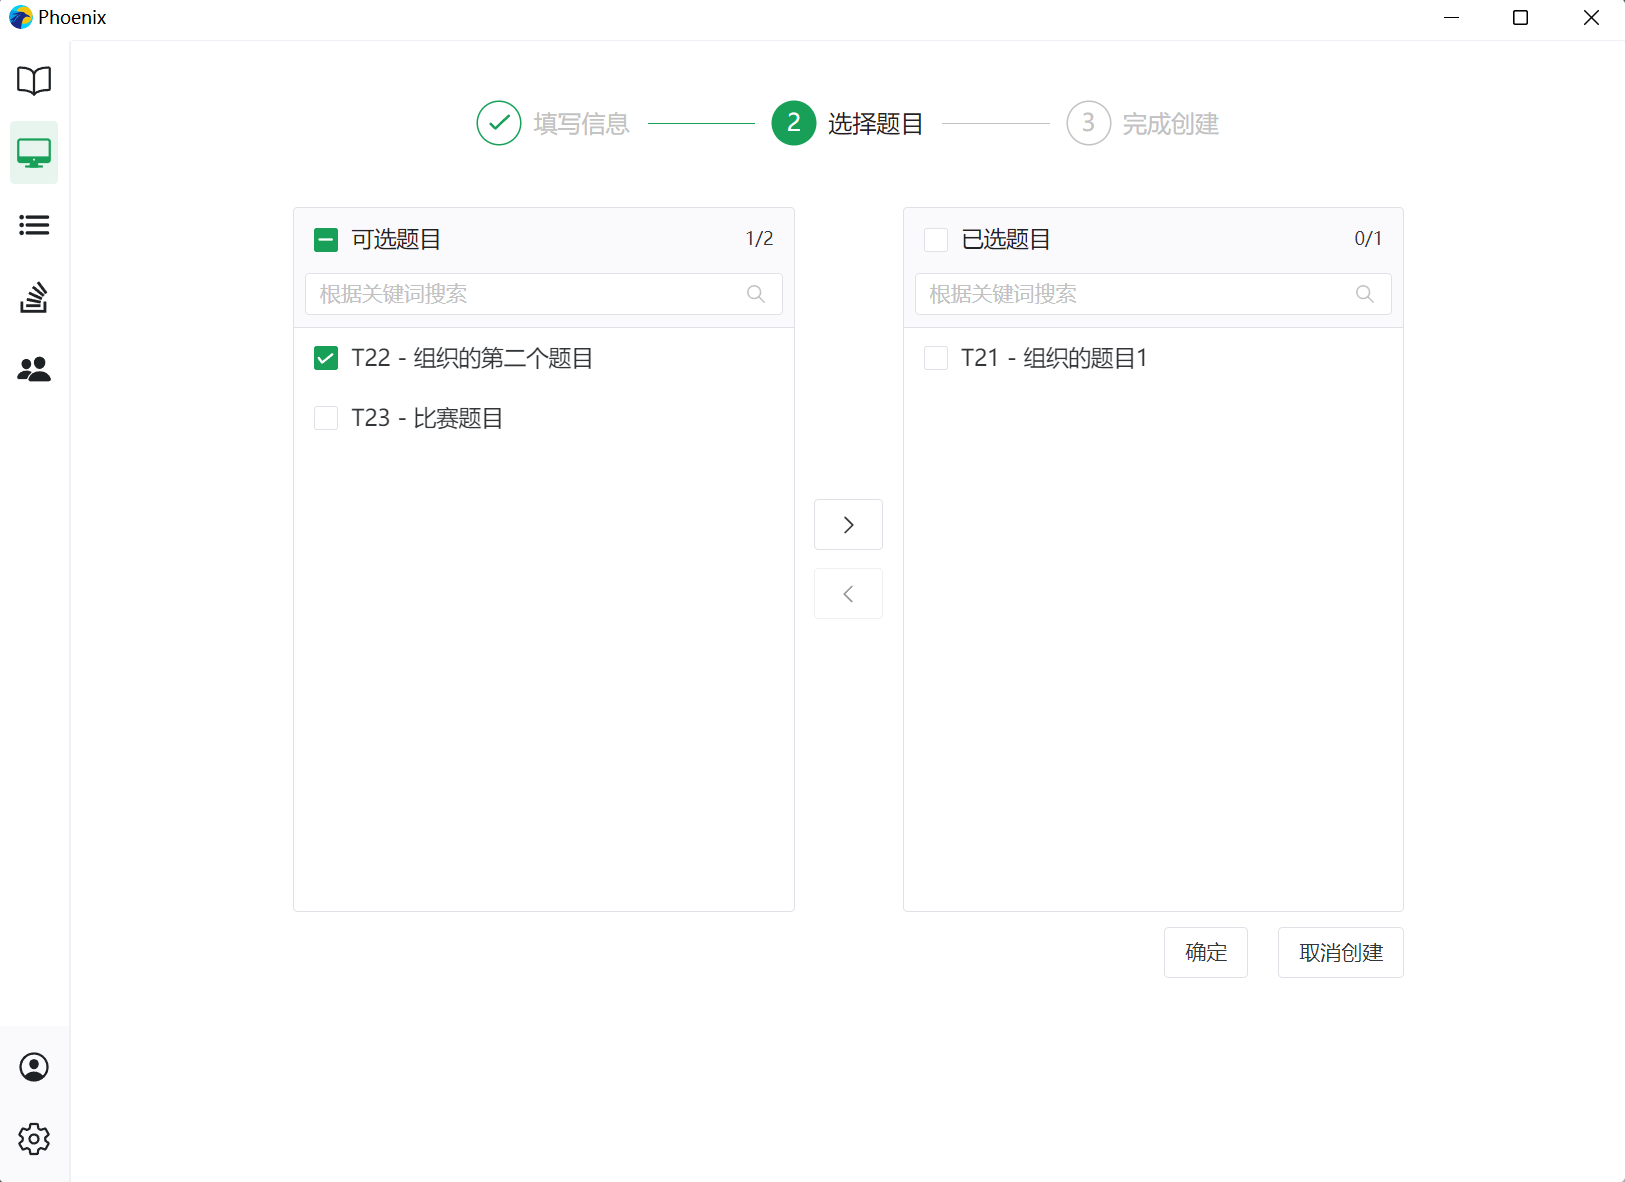
\includegraphics[width=0.7\textwidth]{figure/contest1.png}
    \caption{\textbf{创建比赛页面}}
    \label{fig:contest1}
\end{figure}

到达比赛开始的时间后,具有权限的用户可以对比赛中的题目进行提交。在比赛过程中后台将对用户的提交进行实时排名,用户可以实时看到其他用户的题目通过情况,比赛详情页面如下:

\begin{figure}[H]
    \centering
    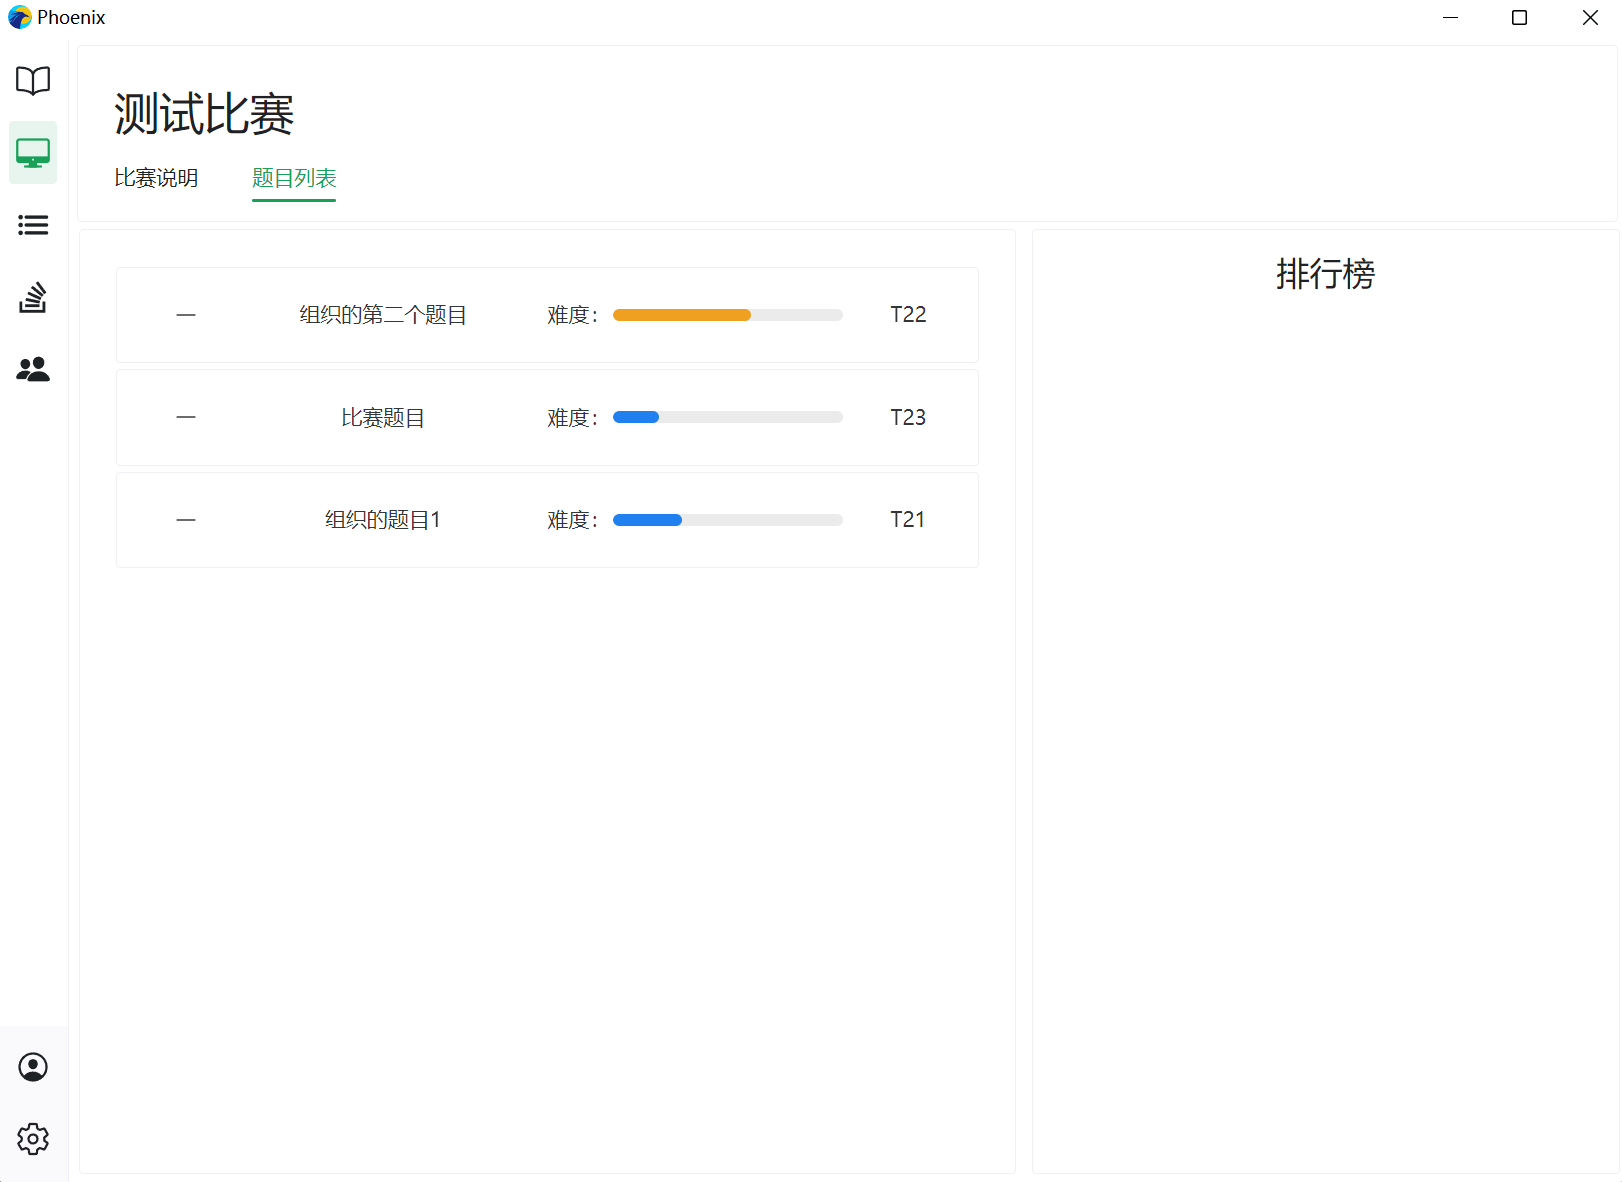
\includegraphics[width=0.7\textwidth]{figure/contest2.png}
    \caption{\textbf{比赛详情页面}}
    \label{fig:contest2}
\end{figure}

\section{论坛版块}

每个组织都有自己的论坛,组织成员可以在论坛内进行交流。论坛内置不同的版块,用于放置不同的讨论内容。论坛内的帖子和评论均可采用Markdown和Latex进行编写,并可插入图片等内容。论坛页面如下:

\begin{figure}[H]
    \centering
    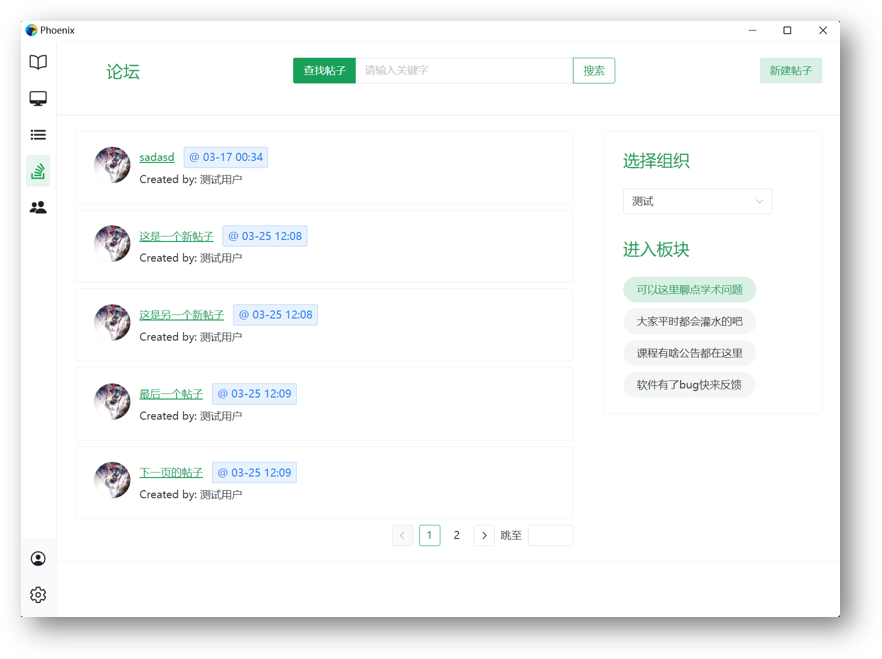
\includegraphics[width=0.7\textwidth]{figure/forum1.png}
    \caption{\textbf{论坛页面}}
    \label{fig:forum1}
\end{figure}
